\subsubsection{Rewrite}

Our sprint 1 code was messy and not well documented, so we did a full rewrite after the submission deadline. This was in the \verb|jottesen_test| folder, named so because it was initially a test of a new pathfinding algorithm. Similarly to \verb|sprint_1|, each robot type had its own class, along with several utility classes. We ended up (mostly) sticking with these utility classes for the rest of the competition, so we will describe them here.

\subsubsection{MapData}

This is really the core of ``what the bot knows''. It stores an array in memory, with one 32-bit int per tile on the map. Below is how we encoded the information in these bits:
\begin{center}
  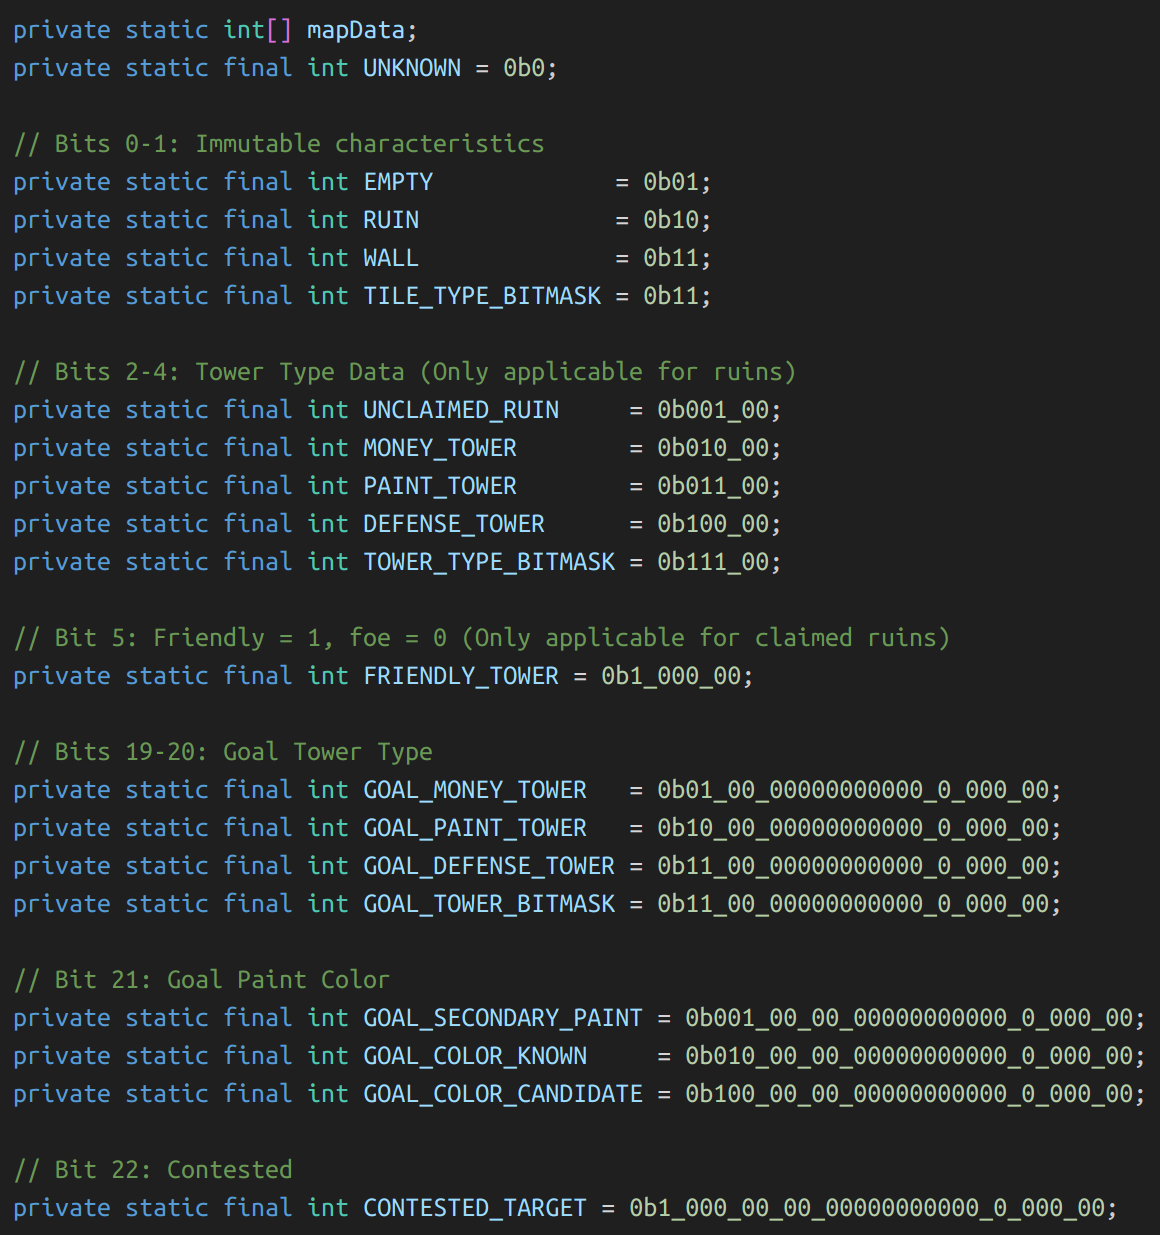
\includegraphics[scale=0.25]{images/mapData_bits.png}
\end{center}
We had plenty of bits left over, and many which were initially used and taken out. Upon spawning, each robot called \verb|MapData.updateAllVisible()| to load all known information about the immediate surroundings into the \verb|mapData| array. Each time the robot moved, it updated only the newly visible tiles. This was a bytecode compromise, since updating all the visible locations was expensive, but only updating newly visible leaves a blind spot around the robot. To help mitigate this, we also kept a list of the known ruins, and updated that list every turn.

\subsubsection{Painter}

We also created a \verb|Painter| class, which heavily relied on the \verb|MapData| class. The \verb|Painter| held the logic for which tiles should be painted, and what color should be used. It used the \verb|GOAL_*| bits from \verb|MapData| to encode these. Whenever we saw a ruin, we set these bits in the $5 \times 5$ area around it. We later did the same with SRPs\footnote{This bot did not bother to paint SRPs, but still heavily outplayed the previous version}. This really streamlined our painting logic, and we didn't have to worry about checking the correct color each time.

\medskip

We also put logic for moppers here, but our moppers were terrible so it isn't really important to discuss. At this point, we still didn't have splashers.

\subsubsection{Communication}

We added the groundwork for our future communication class, however it was not used at all in this iteration. We wrote functions to communicate map symmetry, but did not use them until much later in the competition.

\subsubsection{Pathfinding}

This class was one of the big upgrades of the rewrite\footnote{It was honestly a waste of time since we ended up scrapping it later. It used too much bytecode and was too buggy.}. In the initial bot, we used a pure BugNav algorithm from a previous year, as mentioned previously. This worked, but was inefficient at times. Since we stored the map internally, we could simulate doing BugNav, but have the bot actually take shortcuts.

\medskip

The core idea was that the bot would have some goal target that it was trying to move towards. The algorithm is loosely described below:
\begin{enumerate}
  \item Simulate greedy movement towards the target on the internal \verb|MapData| array. If you hit either the target or an unknown tile, return and follow that path.
  \item If you hit an obstacle, simulate BugNav until you make it past, or you hit an unknown tile.
  \item Repeat the algorithm on the result of the above BugNav.
\end{enumerate}
We managed the target destinations by creating a fixed buffer \verb|Stack| class. Whenever we needed a checkpoint target (found by the BugNav step), we would push it onto the stack. When we reached that target, we popped it off and recalculated the path to the next target. Another useful optimization we used in pathfinding was caching and pre-calculating moves. This let us calculate several moves in advance without wasting a ton of bytecode on recalculations.

\medskip

The main reasons this failed were because of high bytecode cost, greedy search instead of BFS, and bad handling of the case of maximum stack depth of locations. It would outperform our old algorithm in ``easy'' pathfinding scenarios, but would often unpredictably get stuck on the harder situations. Traditional BugNav from XSquare's codebase was a more reliable solution.

\subsubsection{Opening Theory}

Up until this point, we hadn't really considered any type of coordinated effort. Our entire goal was just to build up economy, and if you see any enemies, try and beat them. This is the point we started to consider higher level strategy, so we made a \verb|sprint_2| bot to test our changes against the previous \verb|jottesen_test| and make sure we were in fact making improvements.

\medskip

The goal of the opening is to get a tower-count lead over your opponent. SRPs are not worth it since they take too long to activate, they don't provide enough resources, your team always starts with more than enough chips for towers, and there are always available towers to capture (this is something Teh Devs could've, but never really messed with). In the opening, each tower could spawn two robots before running out of initial paint. The logical choices were either spawning 1 soldier and 1 mopper, or spawning 2 soldiers. 2 soldiers is ideal since together, they could capture a tower without any surrounding paint in 12 turns. However, a mopper would allow the its soldier partner to capture a tower with enemy paint in its pattern. This provides quite the dilemna and was one of the most interesting part of optimizing strategy. 

\medskip

After Sprint 1, we were made aware that rushing with a soldier-pair in the opening was a viable strategy. This provided an elegant solution to the opening dilemna: the soldier pair is better.

\medskip

Each tower spawns 2 soldiers. The first priority of the soldier pair is always to capture an ``uncontested'' ruin\footnote{A ruin with no enemy paint blocking the pattern}. Until the soldiers finished the first ruin, they were in ``opening mode.'' However, in the case that the soldiers only found ruins that were ``contested,'' they would rush. This is theoretically the perfect scenario for rushing since the best counter to rushing is to capture a ruin as fast as possible. However, if every nearby ruin is contested, rushes become stronger since it is more difficult to capture ruins.\\

\medskip

This opening strategy was wildly successful on the ladder. On 90\% of the test maps, the soldier pair would find an uncontested ruin and capture it before turn 20. Our logic didn't result in the soldiers rushing often, but when they did, it was often successful in giving our team a large lead. It wasn't infrequent to see our team with a marginal lead over top teams out of the opening.

\medskip

Our opening strategy remained unchanged after Sprint 2. This lead to some pitfalls. First, requiring the soldiers to pair up meant that if they found an uncontested ruin, they could capture it quicker than if they split up and both found uncontested ruins. However, requiring the soldiers to pair up was very high variance: sometimes, they would miss an obvious ruin since they didn't spread out. Secondly, since rushes happened so infrequently, we never had good logic for what to do after a rush completed, and relied mostly on the rush being disruptive enough to give us a massive lead that we couldn't fumble.


\subsubsection{GoalManager}

The last big change we made before Sprint 2 was introducing the \verb|GoalManager| class. We previously were storing the goal location as a single \verb|MapLocation| and the type as an enum. However, this lead to many problems. Often, ruins would be abandoned when robots went back to get their paint refilled, since they were the only robot that knew it was in progress. After refilling paint, they would act as if they were a new soldier.

\medskip

We decided to use a stack for the goals, giving robots a lot more choice in their intended actions on goals. This ended up being a huge improvement, and we will definitely be bringing this back in future years.

\subsubsection{Paint Towers?}

At some point, we made a change where we built some paint towers. I forgot we did this, but we ended up reverting this decision later. As explained in previous sections, money towers are simply better until you have 4+ SRPs. We did not prioritize SRPs whatsoever, so paint towers didn't make any sense for us.

\subsubsection{Sprint 2 Performance}

The bracket for Sprint 2 can be found \href{https://challonge.com/bc25javasprint2}{here}.

\medskip

We entered the tournament as the 63 seed out of 183 teams, with a rating of 1559. Our first match was a 5-0 win against the 66 seed, ``achromatic'' with a rating of 1551. There was not much of note in these matches, we outplayed them by a wide margin, expanding faster and winning any direct territory battles.

\medskip

Our second match was the opposite, we were against the 2 seed ``Super Cow Powers'' with a rating of 2017. We were no match for them and lost 5-0. They were much more purposeful with their expansion, and we had too many bugs that caused us to sit idle doing nothing.